\chapter{Analisis}
\label{chap: Analsisis}

Berdasarkan hasil studi pustaka yang telah dilakukan, pada bab ini akan dijelaskan hasil analisis
yang berupa spesifikasi dari perangkat lunak, diagram use-case, skenario.

\section{Analisis Perangkat Lunak yang Dibangun}
\label{sec: Analisis Perangkat Lunak yang Dibangun}
Dari pengetahuan yang diperoleh melalui studi pustaka yang dilakukan. Telah ditentukan beberapa analisis untuk membangun Perangkat Lunak Pohon Kurikulum 2018 menggunkan JSON. Berikut beberapa analisis yang telah diambil dari bab 2: 
\begin{itemize}
\item \textbf{Menggunakan \textit{JSON} yang konversikan ke dalam \textit{DOT Language}}\\
Untuk membuat graf harus dilakukan konversi dari\textit{JSON} ke dalam \textit{DOT Language}. \textit{DOT Language} sendiri digunakan untuk menghasilkan graf yang akan menampilkan pohon kurikulum. 

\item \textbf{\textit{JSON} dipakai sebagai data terbuka}\\
\textit{JSON} akan di simpan di \url{github.com}. Tujuannya agar \textit{JSON} menjadi format data terbuka. Setelah disimpan di dalam \textit{github} \textit{JSON} dapat dipakai oleh siapa saja. Karena \textit{github} sendiri merupakan \textit{open source}.

\item \textbf{Perangkat Lunak Menghasilkan Graf Berbentuk Pohon Kurikulum}\\
Perangkat lunak yang akan dibangun akan menghasilkan graf yang berbentuk pohon kurikulum. Pohon kurikulum ini diperlukan agar mahasiswa mengetahui mata kuliah yang akan di ambil di semester baru. 

\item \textbf{Perangkat Lunak akan Menampilkan Mata Kuliah}\\
Perangkat Lunak yang dibangun setelah menghasilkan pohon kurikulum akan menampilkan mata kuliah yang ada di kurikulum baru. Mata Kuliah akan berisi mata kuliah wajib, mata kuliah pilihan, dan mata kuliah pilihan wajib.
\end{itemize}

Struktur \textit{JSON} yang akan digunakan adalah dalam bentuk array yang di dalamnya memiliki objek.  
Objek di dalam JSON ini menjadi acuan dalam membuat pohon kurikulum. Contoh penulisan \textit{JSON} sebagai berikut:

\begin{lstlisting}
[
  {
    "kodeMatkul": "AIF181101",
    "namaMatkul": "Computational Thinking",
    "tempuh": [],
    "lulus": [],
    "bersamaan": [],
    "sks": 3,
    "jenis": "wajib",
    "semester": 1
  }
]
\end{lstlisting}

Pada bentuk di atas \textit{JSON} memiliki beberapa objek sebagai acuan.
\begin{enumerate}
\item \textbf{kodeMatkul}, berisikan kode matakuliah yang akan di ambil di dalam pembuatan pohon kurikulum.
\item \textbf{namaMatkul}, berisikan nama mata kuliah yang ada di semester 1 sampai semester 8.
\item \textbf{tempuh}, berisikan kode mata kuliah yang menunjukan mahasiswa sudah mengambil mata kuliah yang menjadi syarat atau belum. 
\item \textbf{lulus}, \item \textbf{tempuh}, berisikan kode mata kuliah yang menunjukan mahasiswa sudah mengambil mata kuliah yang menjadi syarat dan lulus mata kuliah tersebut.
\item \textbf{bersamaan}, berisikan kode mata kuliah yang menunjukan mahasiswa dapat mengambil mata kuliah yang memiliki syarat bersamaan dengan mata kuliah yang sudah tempuh.
\item \textbf{sks}, menunjukkan berapa banyak tanggungan belajar mahasiswa.
\item \textbf{jenis}, menunjukkan mata kuliah tersebut jenisnya wajib atau pilihan.
\item \textbf{semester}, menunjukkan mata kuliah tersebut ada di semester berapa.
\end{enumerate}

\section{Kebutuhan Data Terbuka}
\label{sec: Kebutuhan Data Terbuka}
~\cite{creativecommons:06:lisensi}

Tujuan utama dari Data Terbuka adalah memaksimalkan penggunaan data seluas-luasnya untuk menciptakan suatu nilai tambah. Untuk mencapai hal tersebut, Data Terbuka memberikan dua komponen dari keterbukaan, yaitu: terbuka secara teknis dan terbuka secara legal. 

Secara sederhana, yang dimaksud dengan data yang terbuka secara legal adalah tidak ada halangan dari sisi aturan atau hukum untuk menggunakan data tersebut. Data boleh dan dapat digunakan oleh siapa saja, untuk tujuan apa saja, kapan saja, tanpa prasyarat apapun, kecuali dengan memberikan atribusi kepada pemilik data. Oleh karena itu, dibutuhkan suatu mekanisme yang jelas untuk mencapai hal-hal tersebut. Salah satu pilihan mekanisme yang bisa digunakan adalah pemberian lisensi kepada data yang hendak dijadikan terbuka secara legal.   

Pembubuhan lisensi atas data diartikan sebagai pemberian hak menggunakan data untuk kepentingan tertentu sesuai dengan syarat dan ketentuan yang tertera di dalam lisensi tersebut tanpa meniadakan hak cipta atas data tersebut. Dengan pemberian lisensi kepada data, data dapat dipergunakan secara mudah (dengan syarat dan ketentuan tertentu) tanpa harus meminta izin melalui mekanisme hak cipta. 

Untuk kebutuhan data terbuka yang bebas biaya dapat menggunakan \textit{github}. Di dalamnya harus menambahkan lisensi untuk pemakaian \textit{github}. Lisensi \textit{Creative Commons} adalah salah satu lisensi publik yang memungkinkan pemilik karya untuk mendistribusikan dan memperbolehkan penggunaan karyanya secara bebas. Ada beberapa tipe lisensi \textit{Creative Commons} yang dapat dipergunakan ketika seorang pemilik karya hak cipta hendak mendistribusikan dan memperbolehkan penggunaan atas karyanya.  

Tipe-tipe lisensi Creative Commons antara lain:
\begin{enumerate}
\item Attribution (BY) \\
Mengizinkan orang lain untuk menyalin, mendistribusikan, menampilkan, serta membuat karya turunan berdasarkan suatu karya hanya jika orang tersebut memberikan penghargaan pada pencipta atau pemberi lisensi dengan cara yang disebutkan dalam lisensi.
\item ShareAlike (SA) \\
Mengizinkan orang lain untuk mendistribusikan suatu karya turunan hanya di bawah suatu lisensi yang identik dengan lisensi yang diberikan pada karya aslinya. 
\item Non-Commercial (NC) \\
Mengizinkan orang lain menyalin, mendistribusikan, menampilkan, serta membuat karya turunan berdasarkan suatu karya hanya untuk tujuan non-komersial.
\item Non-Derivative (ND) \\ 
Mengizinkan orang lain menyalin, mendistribusikan, dan menampilkan hanya salinan sama persis suatu karya, bukan karya turunan yang berdasarkan karya tersebut.   
\end{enumerate}

Dari tipe-tipe lisensi di atas, maka lisensi \textit{Creative Commons} yang paling tepat untuk digunakan untuk Data Terbuka di Indonesia adalah lisensi \textit{Creative Commons by Attribution} (CC-BY) dikarenakan lisensi CC-BY inilah yang paling mendekati persyaratan keterbukaan dari Data Terbuka, yaitu: pengguna dapat mendistribusikan data dan menggunakan data secara bebas baik untuk kepentingan komersil, maupun non-komersil tanpa syarat kecuali dengan memberikan atribusi kepada pemilik data.

Selain itu, lisensi CC-BY ini bisa dikatakan sebagai lisensi publik paling mudah dipakai untuk memaksimalkan penggunaan atas data tanpa membuat pengguna data khawatir atas status legalitas dari penggunaan data dan akibat dari penggunaan data tersebut.

\section{Spesifikasi Perangkat Lunak yang Dibangun}
\label{sec: Spesifikasi Perangkat Lunak yang Dibangun}

Berawal dari pengetahuan yang diperoleh melalui studi pustaka yang telah dilakukan, maka selanjutnya
menentukan spesifikasi website perangkat lunak yang akan dibangun. Perangkat lunak ini hanya
memiliki beberapa spesifikasi, antara lain:
\begin{itemize}
\item Menggunakan \textit{JSON} 
\item Menggunakan \textit{DOT Language}
\item Visualisasi menggunakan \textit{viz.js}
\item Memakai data terbuka
\item Memakai graf
\end{itemize}

\subsection{Diagram Use Case dan Skenario}
\label{sec: Diagram Use Case dan Skenario}

\begin{figure}[H]
		\centering
		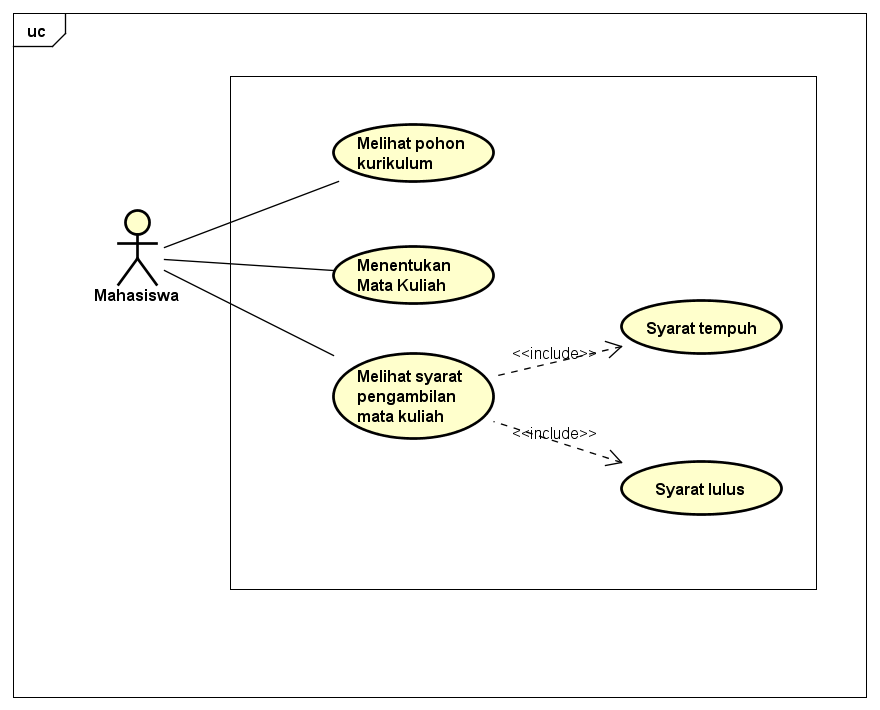
\includegraphics[scale = 0.5]{UseCasePohon.png}
		\caption{Use Case Pohon Kurikulum}
		\label{fig: Use Case Pohon Kurikulum}
\end{figure}	

Berikut keterangan dan skenario dari Gambar \ref{fig: Use Case Pohon Kurikulum}:
\begin{enumerate}
\item Nama \textit{use case} : Melihat Pohon Kurikulum \\
	  Aktor : Mahasiswa 
	  Deskripsi :  Aktor melihat isi pohon kurikulum 
	  Prakondisi : Aktor belum mengetahui pohon kurikulum baru 
	  Skenario normal : Aktor melihat pohon kurikulum
	  Eksepsi : Aktor telah mengetahui pohon kurikulum yang di pakai di kurikulum baru
	  
\end{enumerate}


